\documentclass{article} % JASA requires 12 pt font for manuscripts
%\usepackage{JASA_manu}        % For JASA manuscript formatting

% for citations
\usepackage[authoryear]{natbib} % natbib required for JASA
\usepackage[colorlinks=true, citecolor=blue, linkcolor=blue]{hyperref}

%\definecolor{Blue}{rgb}{0,0,0.5}
\newcommand{\hh}[1]{{\color{orange} #1}}

% fonts
%\usepackage{kpfonts}

% for figures
\usepackage{graphicx}
\graphicspath{{figures/}}

% help with editing and coauthoring
\usepackage{todonotes}

% title formatting
\usepackage[compact,small]{titlesec}

% page formatting
\usepackage[margin = 1in]{geometry}
\usepackage[parfill]{parskip}

% line spacing
\usepackage{setspace}
\doublespace

% For math typsetting
\usepackage{bm}
\usepackage{amstext}
\usepackage{amssymb}
\usepackage{amsmath}
\usepackage{amsfonts}
\usepackage{multirow}

% A few commands to make typing less tedious
\newcommand{\inv}{\ensuremath{^{-1}}}
\newcommand{\ginv}{\ensuremath{^{-}}}
\newcommand{\trans}{\ensuremath{^\prime}}
\newcommand{\var}{\ensuremath{\mathrm{Var}}}
\newcommand{\cov}{\ensuremath{\mathrm{Cov}}}


\title{Simulation-Based Diagnostics for Hierarchical Linear Models: A Graphical Approach}

%\author{Adam Loy and Heike Hofmann}
%	Department of Statistics\\
%	Iowa State University\\
%	Ames, IA 50011-1210
%}

\begin{document}
\maketitle
\todo[inline]{What names should we put on this chapter for the dissertation?}
%------------------------------------------------------------------------------------
\section{Introduction}
%------------------------------------------------------------------------------------

Hierarchical linear models (i.e., multilevel models, linear mixed effects models, random coefficient models) are versatile models that allow for dependence expected when data are organized in hierarchical structures---such data structures are especially common in social science research where studies often focus on responses from human subjects. Examples of these structures include when subjects are naturally grouped by organization (e.g., student within schools), geography (e.g., voters within states), and interviewer (e.g., respondents assigned to an interviewer). The additional flexibility offered by these models to incorporate data from each level of the data hierarchy and allow for dependencies between individuals within the same group complicates model exploration and verification. More specifically, residual plots often display noticeable patterns, but these patterns are often artifacts of model estimation rather than indications of lack of fit. To mitigate the risk of detecting such artifacts we suggest a graphical simulation-based approach to model checking that makes use of the protocols from visual inference \citep{Buja:2009hp}.


%------------------------------------------------------------------------------------
\section{Hierarchical linear models}\label{sec:hlms}
%------------------------------------------------------------------------------------

\subsection{Notation and formulation}
%------------------------------------------------------------------------------------
In this paper we consider the continuous response hierarchical linear model
%
\begin{equation}\label{eq:hlm}
	\underset{(n_i \times 1)}{\bm{y}_i} = \underset{(n_i \times p)}{\bm{X}_i} \ \underset{(p \times 1)}{\bm{\beta}} + \underset{(n_i \times q)}{\bm{Z}_i} \ \underset{(q \times 1)}{\bm{b}_i} + \underset{(n_i \times 1)}{\bm{\varepsilon}_i}
\end{equation}
%
where $\bm{y}_i$ is the vector of outcomes for the $n_i$ level-1 units in group $i=1, \ldots, m$, $\bm{X}_i$ and $\bm{Z}_i$ are design matrices for the fixed and random effects, respectively, $\bm{\beta}$ is a vector of fixed effects governing the global mean structure, $\bm{b}_i$ is a vector of random effects governing the between-group covariance structure, and $\bm{\varepsilon}_i$ is a vector of level-1 error terms governing the within-group covariance structure. We further assume that the random effects, $\bm{b}_i$, are a random sample from $\mathcal{N}(\bm{0},\ \bm{D})$ that are independent from the level-1 error terms, $\bm{\varepsilon}_i$, which we assume are a random sample from $\mathcal{N}(\bm{0},\ \bm{R}_i)$. 
Inference typically centers around either the marginal or conditional distribution of $\bm{y}_i$, depending whether global or group-specific questions are of interest.
Based on model \eqref{eq:hlm} the marginal distribution of $\bm{y}_i$ is given by
%
\begin{equation}\label{eq:marginalmod}
\bm{y}_i \sim \mathcal{N}\left(\bm{X}_i\bm{\beta},\ \bm{V}_i \right)
\end{equation}
%
where $\bm{V}_i = \bm{Z}_i \bm{DZ}_i + \bm{R}_i$, and the conditional distribution of $\bm{y}_i$ given $\bm{b}_i$ is given by
%
\begin{equation}\label{eq:conditionalmod}
\bm{y}_i | \bm{b}_i \sim \mathcal{N}\left(\bm{X}_i\bm{\beta} + \bm{Z}_i \bm{b}_i, \ \bm{R}_i \right)
\end{equation}
%


\subsection{Residuals}
%------------------------------------------------------------------------------------
As with the classical linear model with uncorrelated errors, residuals are central to exploring the fit of a hierarchical linear model. For hierarchical linear models residual analysis is complicated by the fact that there are numerous quantities that can be defined as \emph{residuals}, with each residual quantity being associated with different aspects of the model. Two fundamental residuals for model checking include
%
\begin{itemize}
\item the level-1 residuals (i.e., the conditional residuals) $\widehat{\bm{\varepsilon}}_i = \bm{y}_i - \bm{X}_i \widehat{\bm{\beta}} - \bm{Z}_i \widehat{\bm{b}}_i$,

\item and the level-2 residuals (i.e., the predicted random effects) $\widehat{\bm{b}}_i$
\end{itemize}
%
where, assuming $\bm{V}$ is known
\begin{equation}\label{eq:glsb}
	\widehat{\bm{\beta}} = 
	\left(\sum^m_i \bm{X}\trans_i \bm{V}^{-1}_i \bm{X} \right)^{-1} 
	\sum^m_i \bm{X}_i\trans \bm{V}_i\inv \bm{y}_i,
\end{equation}
and
\begin{equation}\label{eq:eb}
	\widehat{\bm{b}}_i = \bm{D} \bm{Z}_i\trans \bm{V}_i^{-1} 
	\left(\bm{y}_i - \bm{X}_i \widehat{\bm{\beta}} \right)
\end{equation}
%
In practice $\bm{V}$ is unknown, so estimates for $\bm{D}$ and $\bm{V}$ are used in the above equation. These estimates are commonly found through maximum likelihood (ML) or restricted maximum likelihood (REML).

\subsection{Conventional practices for model selection and model checking}
%------------------------------------------------------------------------------------

\subsubsection{Model selection}
%------------------------------------------------------------------------------------
It is standard practice to use either a $t$-test or a likelihood ratio test to test whether a fixed effect is significant in a hierarchical linear model. More generally, likelihood ratio tests can be used to compare nested models. One statistical model is nested within another when the \emph{larger model} contains all components included in the \emph{smaller model}, with respect to both fixed and random effects, as well as some additional component(s). For example, the larger model could differ by including additional fixed effects, or by including additional random effects. 

Statistical software has made performing $t$-tests for fixed effects simple, but more thought is often required when performing a likelihood ratio test. More specifically, likelihood ratio tests can only be used with nested models fit by REML if they only differ with respect to their random effects \todo{Would components be more clear?} as the restricted log likelihood contains a term that changes with $\bm{X}_i$ \citep[c.f.,][Section 2.2.5]{Pinhiero:2000vf}. Nested models fit by ML do not have this restriction, so likelihood ratio tests can be used to test both the fixed and random effects. Additional complications arise in the computation of a $p$-value for the likelihood ratio test for covariance parameters on the boundary of the parameter space. In this case, the reference distribution is not $\chi^2$ with degrees of freedom equal to the difference in the number of parameters, but is rather a 50:50 mixture of $\chi^2$ distributions \citep{Self:1987wb, Stram:1994wd}. For example, when testing $q$ versus $q + 1$ random effects, the reference distribution is a 50:50 mixture of $\chi^2_q$ and $\chi^2_{q+1}$.

\subsubsection{Model checking}
%------------------------------------------------------------------------------------


%------------------------------------------------------------------------------------
\section{Visual inference}\label{sec:vi}
%------------------------------------------------------------------------------------
In order to develop graphical model diagnostics as substitutes for statistical tests of model assumptions, we work within a rigorous inferential framework. \cite{Gelman:2004gg} formulates a visual analog of simulation-based model diagnostics in which a visualization of an aspect of the model is compared to data generated under the model. \cite{Buja:2009hp} extend this idea, proposing two protocols that formalize a rigorous inferential framework for testing visual discoveries. In this section we outline the lineup protocol.

Classical statistical inference consists of 
\begin{enumerate}
	\item formulating a null and alternative hypothesis,
	\item calculating a test statistic,
	\item comparing the test statistic to a reference (null) distribution,
	\item and calculating a $p$-value from on which we base our conclusion.
\end{enumerate}
Following \citeauthor{Buja:2009hp}, each of these components has a direct analog in visual inference. \hh{As we will apply visual inference for model diagnostics, we want to highlight these parallels in this framework: the null  hypothesis corresponds to some assumption about the model, such as e.g.~homogeneity of residual variance,
while
the alternative hypothesis encompasses any violation of this model assumption. For visual inference, the test statistic corresponds to a plot  that displays the model assumption and allows the observer to distinguish between scenarios under null and alternate hypothesis. 
A plot of data generated consistently with the null hypothesis is called a null plot. The set of all null plots makes the reference distribution. 
If the model assumption holds, i.e.  under the null hypothesis, the plot of the observed data is indistinguishable from the null plots. 
In the lineup protocol the true plot is randomly embedded among a number of null plots. 
This allows for the estimation of a $p$-value associated with a lineup
%similar to that of permutation tests---if the true plot is distinguishable from a group of $m$ null plots, we would reject the null hypothesis with a $p$-value of $1 / (k + 1)$.
based on an assessment  by human observers: let $x$ be the number of observers, out of $N$, who chose the true plot from the lineup. The $p$-value is then given as the probability that at least as many observers chose the true plot given that the true plot is not any different from the other plots in the lineup. Under the null hypothesis the probability for choosing the true plot is $1/m$, and $X$, the number of observers choosing the true plot is distributed according to a Binomial distribution: $X \sim B_{N, p}$. The $p$-value is then estimated as
\begin{equation}\label{eqn.pvalue}
\widehat{p\text{-value}} = P(X \ge x) = \sum_{k= x}^N {N \choose k} \left(1/m\right)^k \left(1 - 1/m\right)^{N-k}.
\end{equation}
Similarly, the lineup protocol also allows for an assessment of the power of a lineup \cite{mahbub:2013} as the probability that in $N$ independent evaluations observers choose the true plot at least $x_\alpha$ times:
\begin{equation}\label{eqn:power}
\widehat{Power} = {Power}_{N} = 1 - F_{X} (x_{\alpha} - 1),
\end{equation}
where $F_X$ is the distribution of $X$ and $x_\alpha$ is the critical value for a given significance level of $\alpha$, i.e. $P(X \ge x_{\alpha}) \le \alpha$. $X$ is composed of the sum of $N$ observers' (binary) decisions $X_i \sim B_{1, p_i}$.  $p_i$ is the probability that individual $i$ chooses the true plot, which  depends both on the strength of the signal in the true plot and an individual's visual ability.
Assessing an individual's ability requires that an individual evaluates multiple lineups. If that is not possible, we have to assume that all individuals share the same ability, and the power calculation of eqn.~(\ref{eqn:power}) simplifies to $1 - B_{N, \hat{p}}(x_\alpha-1)$, where $\widehat{p} = x/N$ is an estimate for the probability that an individual chooses the true plot.



}

%------------------------------------------------------------------------------------
\section{Visual inference for hierarchical linear models}
%------------------------------------------------------------------------------------

In this section we discuss how visual inference can be implemented to conduct common tests for hierarchical linear models and to avoid misinterpreting residual plots. 

\subsection{Model selection}
%------------------------------------------------------------------------------------

%\subsubsection{Conventional hypothesis tests}
%%------------------------------------------------------------------------------------
%It is standard practice to use either a $t$-test or a likelihood ratio test to test whether a fixed effect is significant in a hierarchical linear model. More generally, likelihood ratio tests can be used to compare nested models. One statistical model is nested within another when the \emph{larger model} contains all components included in the \emph{smaller model}, with respect to both fixed and random effects, as well as some additional component(s). For example, the larger model could differ by including additional fixed effects, or by including additional random effects. 
%
%Statistical software has made performing $t$-tests for fixed effects simple, but more thought is often required when performing a likelihood ratio test. More specifically, likelihood ratio tests can only be used with nested models fit by REML if they only differ with respect to their random effects \todo{Would components be more clear?} as the restricted log likelihood contains a term that changes with $\bm{X}_i$ \citep[c.f.,][Section 2.2.5]{Pinhiero:2000vf}. Nested models fit by ML do not have this restriction, so likelihood ratio tests can be used to test both the fixed and random effects. Additional complications arise in the computation of a $p$-value for the likelihood ratio test for covariance parameters on the boundary of the parameter space. In this case, the reference distribution is not $\chi^2$ with degrees of freedom equal to the difference in the number of parameters, but is rather a 50:50 mixture of $\chi^2$ distributions \citep{Self:1987wb, Stram:1994wd}. For example, when testing $q$ versus $q + 1$ random effects, the reference distribution is a 50:50 mixture of $\chi^2_q$ and $\chi^2_{q+1}$.


%\subsubsection{Visual hypothesis tests}
%------------------------------------------------------------------------------------
Visual tests provide an alternative to conventional hypothesis tests that does not have limitations based on whether ML or REML was used to fit the model since they do not rely on the (restricted) log likelihood. Additionally, the $p$-value from a visual test is calculated using the Binomial distribution, which does not require adjustments to an asymptotic distribution. Rather, visual tests depend on the plot chosen, the number of alternatives, and the number of viewers. Below we discuss visual tests useful in model selection.

\paragraph{Fixed effects.} To test the significance of a fixed effect, we suggest using a plot comparing a residual quantity from the model without the variable of interest and the values of that variable. The residual used depends on the level at which the variable of interest enters the model---if the variable enters at the observation-level (level-1), then the level-1 residuals should be used; if the variable enters at the group level, then the predicted random effects associated with that group should be used. Additionally, the type of plot depends on the variable type---if a continuous variable is targeted, then a scatterplot with a smoother should be used; if a discrete variable is targeted, then side-by-side boxplots should be used.

%To illustrate the use of visual tests for fixed effects...\todo{Choose a data set!}


\paragraph{Random effects.} Tests of the random part of a hierarchical model focus on two questions---(1) whether a marginal random effect improves the model and (2) whether allowing the random effects to be correlated improves the model---which require the use of different plots to determine an answer. To answer the first question, we suggest plots comparing the response and the explanatory variable of interest using appropriate (often linear) smoothers for each group. Scatterplots comparing the predicted random effects can be used to answer the second question.


\paragraph{Example.}
To illustrate the use of visual inference for tests of the fixed effects and random effects (i.e., covariance parameters) we...


\begin{figure}
	\centering
	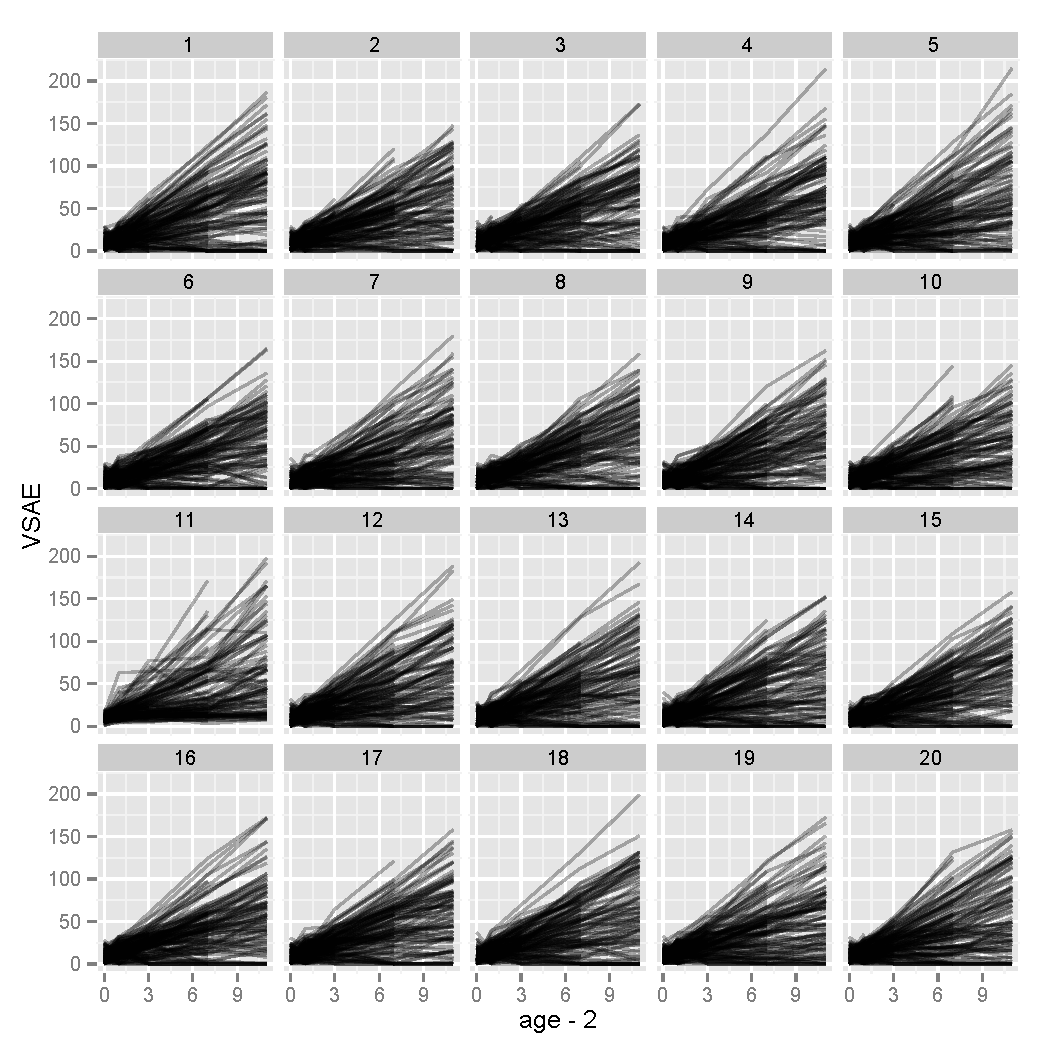
\includegraphics[width=\textwidth]{autism_ranef1_true11.pdf}
	\caption{\label{fig:lineup-ranef1} These 20 plots display a child's VSAE trajectory. Which is the real plot?}
\end{figure}

\begin{figure}
	\centering
	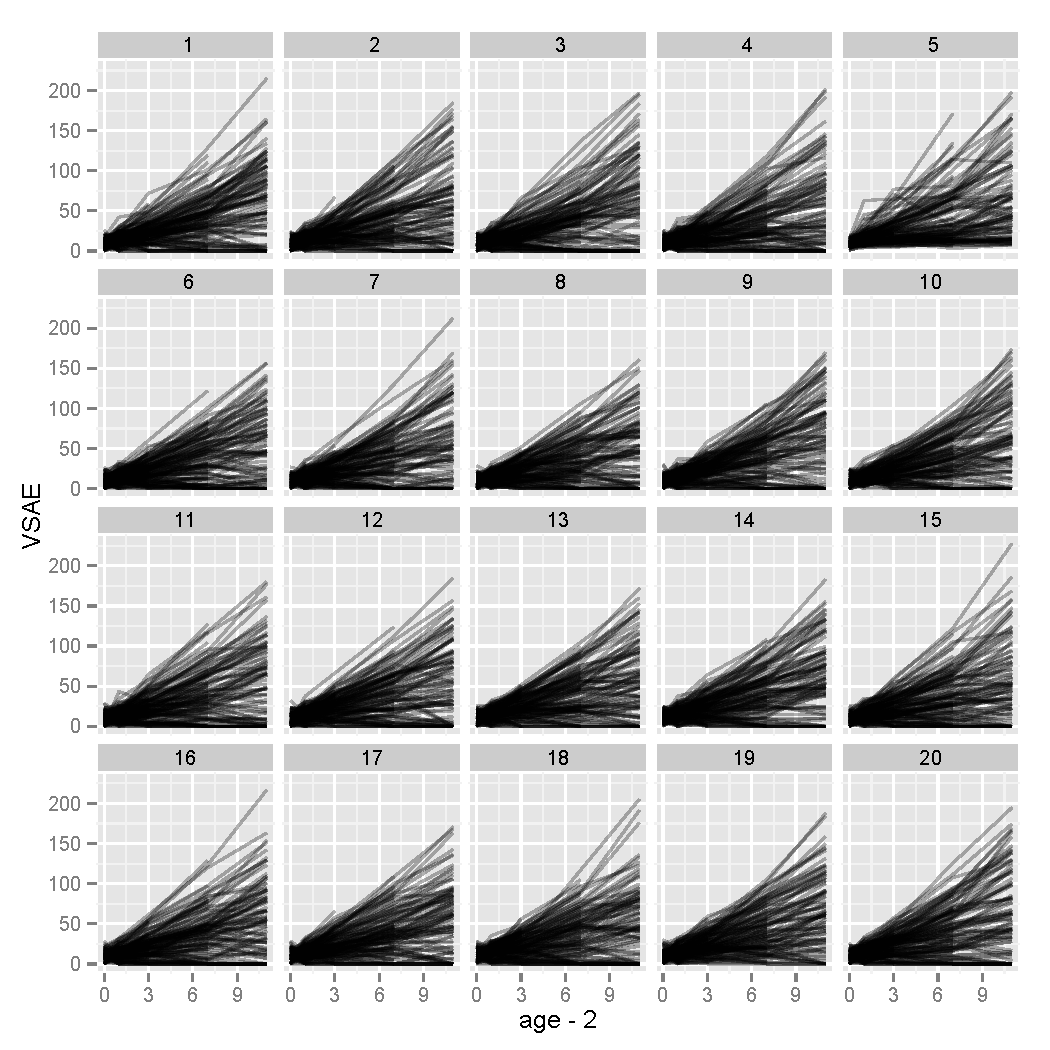
\includegraphics[width=\textwidth]{autism_ranef2_true5.pdf}
	\caption{\label{fig:lineup-ranef2} These 20 plots display a child's VSAE trajectory. Which is the real plot?}
\end{figure}

\begin{figure}
	\centering
	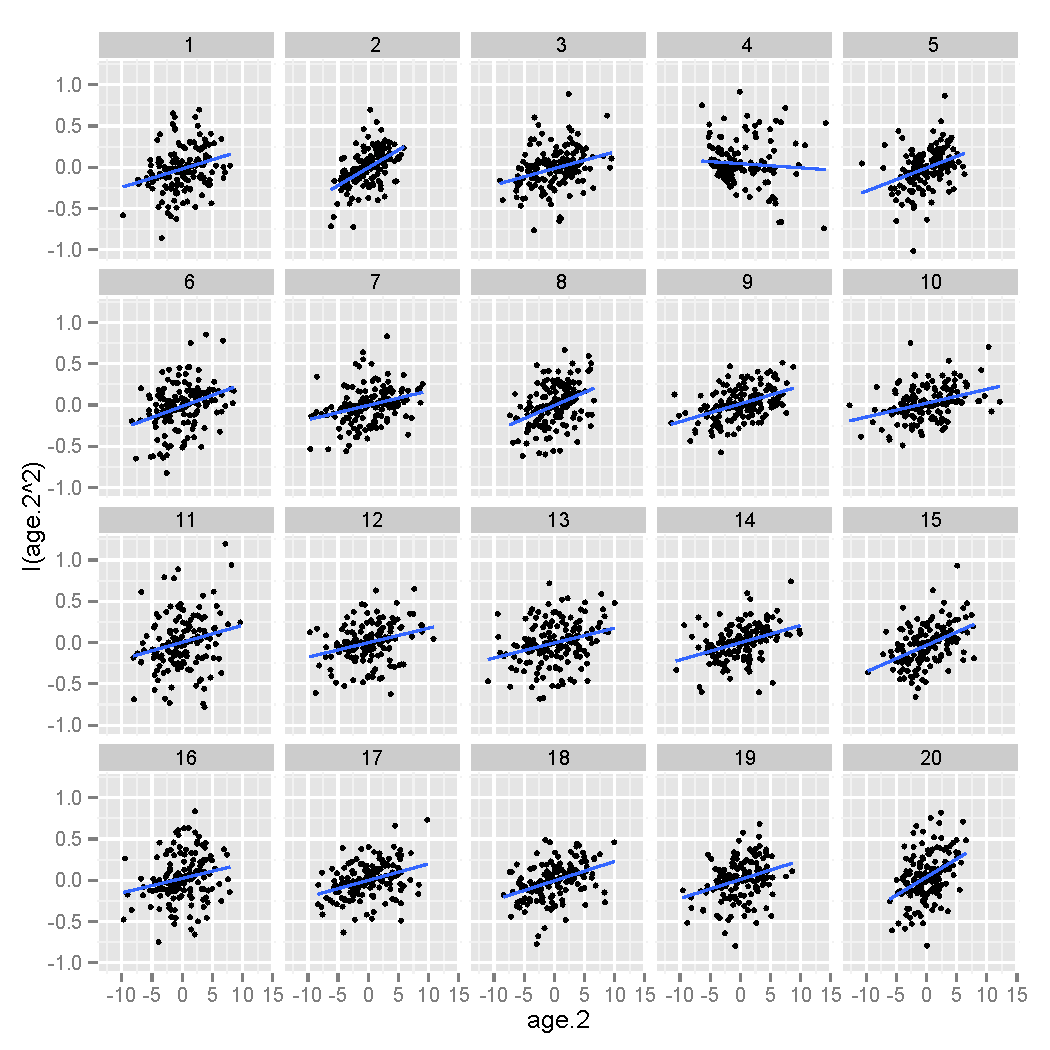
\includegraphics[width=\textwidth]{autism_ranef3_true4.pdf}
	\caption{\label{fig:lineup-ranef3} These 20 plots compare the predicted random intercept and slope from model XX. Which is the real plot?}
\end{figure}

\begin{figure}
	\centering
	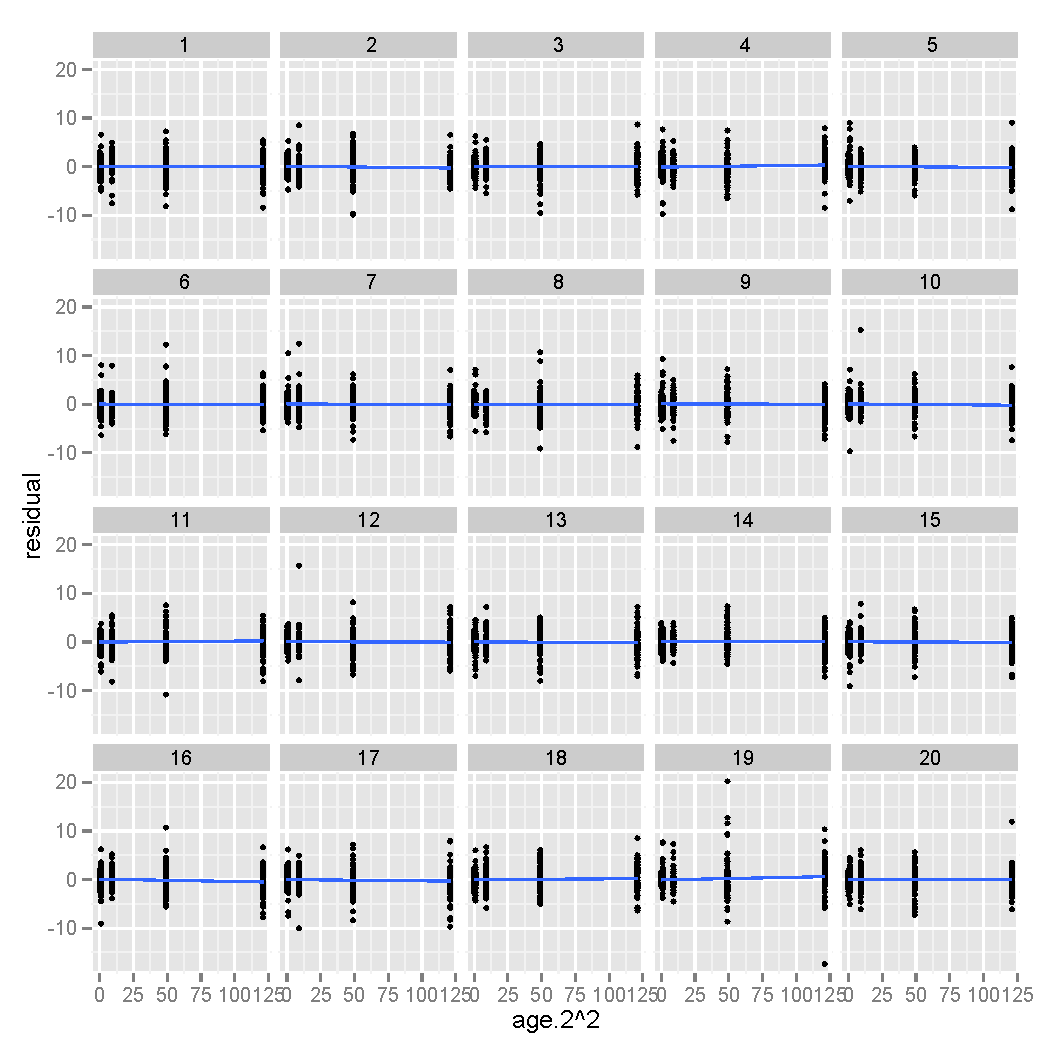
\includegraphics[width=\textwidth]{autism_agesq_true19.pdf}
	\caption{\label{fig:lineup-agesq} These 20 plots show the level-1 residual against age squared. Which is the real plot?}
\end{figure}

\begin{figure}
	\centering
	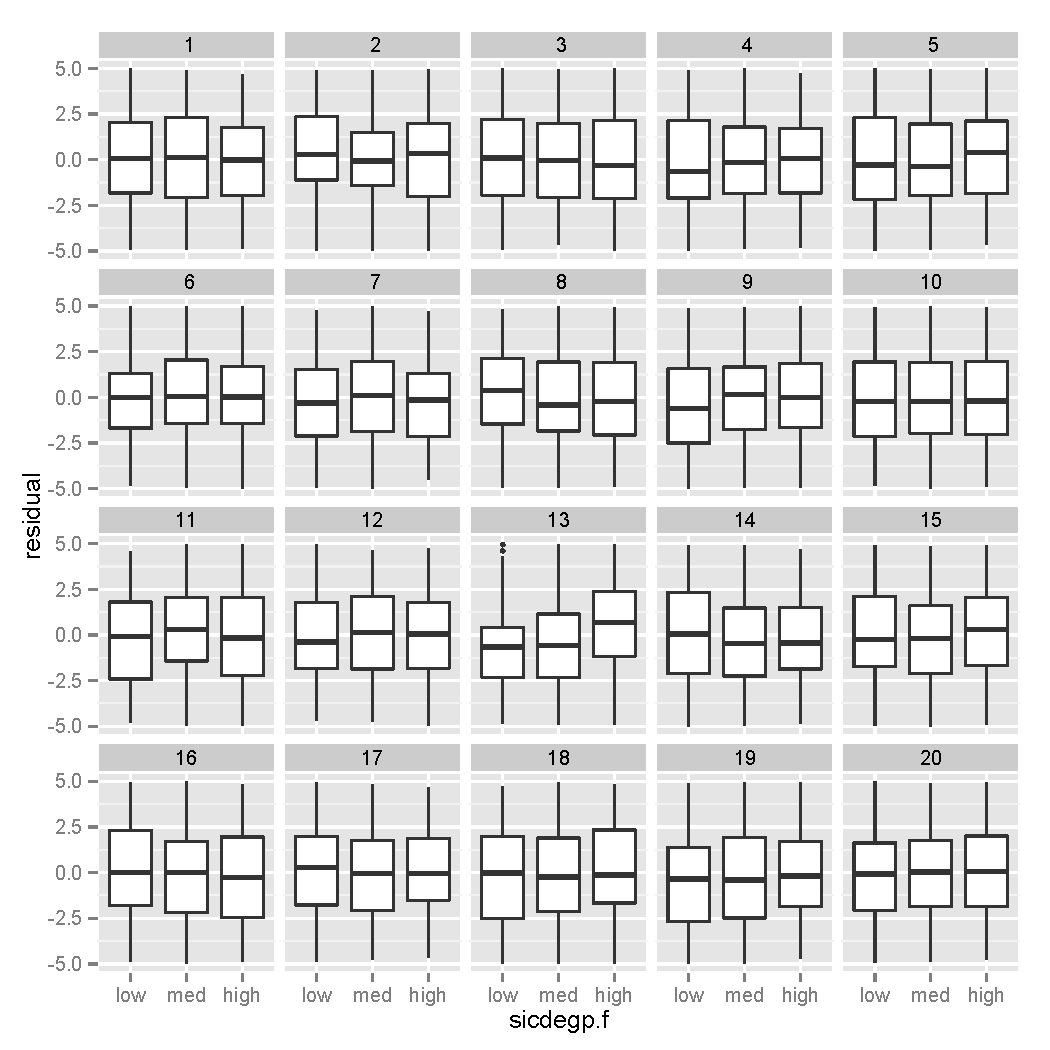
\includegraphics[width=\textwidth]{autism_sicdegp_true13.pdf}
	\caption{\label{fig:lineup-ranef1} These 20 plots show the level-1 residuals against SICDEGP. Which is the real plot?}
\end{figure}

\paragraph{Comparing non-nested models.}
%------------------------------------------------------------------------------------
The conventional hypothesis tests require that the models being compared are nested. If two non-nested models are being considered visual inference can be used to investigate the goodness-of-fit of each model. While this comparison does not directly compare the two models, the results of such an investigation will provide evidence supporting one model over...

\todo[inline]{Does this paragraph belong here? or with model checking?}

\subsection{Model checking}
%------------------------------------------------------------------------------------

Include:
\begin{itemize}
\item Checks for level-1 and -2 heteroscedasticity -- cyclone plots, residuals vs. predictors
\item Linearity

\end{itemize}


\todo[inline]{Below is a list of some initial ideas.}
%------------------------------------------------------------------------------------
\section{Examples}
%------------------------------------------------------------------------------------
Applications of hierarchical models:
\begin{itemize}
\item Education -- students nested in classes nested in schools
\item Interviewer research -- respondents nested in interviewer (Hox 1994)
\end{itemize}

Situations to consider:
\begin{itemize}
\item Residual analysis
	\begin{itemize}
	\item Unbalanced sample sizes introduces structure
	\item Using raw rather than standardized residuals can introduce structure
	\item This could help avoid using theoretical cutoffs for statistics used in the detection of outliers and influential points. \cite{Longford:2001wy} discusses numeric simulation-based diagnostics for outlier and makes some good points about how the theoretical distributions of these statistics are: (1) hard to calculate theoretically in many situations; (2) are based on a unit being randomly selected, as opposed to selected after an inspection of the data.
	\end{itemize}

\item Comparison of random effects -- \cite{Morrell:2000ve} discuss lines in plots of random effects appear when there are groups with a large amount of pooling (shrinkage)

\item Exploratory modeling
	\begin{itemize}
	\item Considering a variable for inclusion in the model as a fixed effect
	\item The need for/utility of additional random effects
	
	\end{itemize}


\end{itemize}

%------------------------------------------------------------------------------------
\section{Discussion}
%------------------------------------------------------------------------------------


%------------------------------------------------------------------------------------
%------------------------------------------------------------------------------------

\bibliographystyle{apalike}
\bibliography{hlmviz_bib}

\end{document}